%!TEX root = ../thesis.tex

\chapter{Frameworks and tools}

\ifpdf
    \graphicspath{{Chapters/Figs/Raster/}{Chapters/Figs/PDF/}{Chapters/Figs/}}
\else
    \graphicspath{{Chapters/Figs/Vector/}{Chapters/Figs/}}
\fi


%********************************** % Section  **************************************
\section{PikeOS}
A trusted Operating System, capable of providing isolation among partitions is crucial for mixed-criticality systems. PikeOS \cite{PikeOS} is a commercial operating system from SYSGO AG, designed in early 2002 to address the needs of a kernel targeting safety and security applications. It uses a separation micro-kernel architecture and provides a hypervisor model at its core. Moreover, PikeOS hypervisor has been certified for all relevant certification standards including DO-178C, IEC 61508, EN 50128, EN 62304, and ISO 26262 coming from the fields of Aerospace/Defense, Automotive, Transportation and Industry/IoT.
\par The micro-kernel architecture allows the OS to be used in resource constrained devices like embedded systems. It supports single and multi-core processor architectures with both models: AMP (Asymmetric Multi-Processing) and SMP (Symmetric Multi-Processing).

\paragraph{}PikeOS includes \emph{CODEO}, an Eclipse-based IDE that provides several functionalities such as guided configuration, compilers, assemblers, remote debugging, application deployment, target monitoring, and timing analyses.

\subsection{Hypervisor general overview}
The PikeOS Hypervisor offers a performance optimized para-virtualization, meaning that the OS presents a software interface to virtual machines that are aware of the virtualization level.

\paragraph{} The PikeOS Microkernel consists of a generic part (CPU architecture dependent) called \emph{Architecture Support Package} (ASP) and a platform dependent part called \emph{Platform Support Package} (PSP): together they form the \emph{Board Support Package} (figure \ref{fig:pikeosarch}). 
The PikeOS Microkernel (with the ASP) is the only component that runs with supervisor privileges. It provides:
\begin{itemize}
\item Hardware abstraction
\item Spatial and temporal separation among partition
\item Communication primitives
\end{itemize}
The \emph{PikeOS System Software} (PSSW) component is the first user space application launched by the PikeOS Microkernel, it performs some initialization and, at run-time, acts as a server providing services like communications, file system access, health monitoring and partition/process management to the applications.

\subsection{Personalities}
In PikeOS guest operating systems, runtime environments or API are called \emph{personalities}. They run on top of the hypervisor in a non-privileged mode as shown in fig \ref{fig:pikeosarch}. Personalities included are:
\begin{itemize}
\item AUTOSAR
\item Android
\item Embedded Linux
\item Native PikeOS
\end{itemize}
Moreover, regarding the runtime environments:
\begin{itemize}
\item Ada
\item AFDX (Avionics Full-Duplex Switched Ethernet)
\item ARINC-653 (Avionics Application Standard Software Interface)
\item Certified POSIX
\item RTEMS (Real-Time Executive for Multiprocessor Systems)
\item Real Time JAVA
\end{itemize}
Other personalities are supported through SYSGO partners.
\par These guests are contained inside a Virtual Machine with their memory space, resources and application set. Applications hosted on one virtual machine run completely independently of those in the others. 

\begin{figure}[htbp] 
\centering    
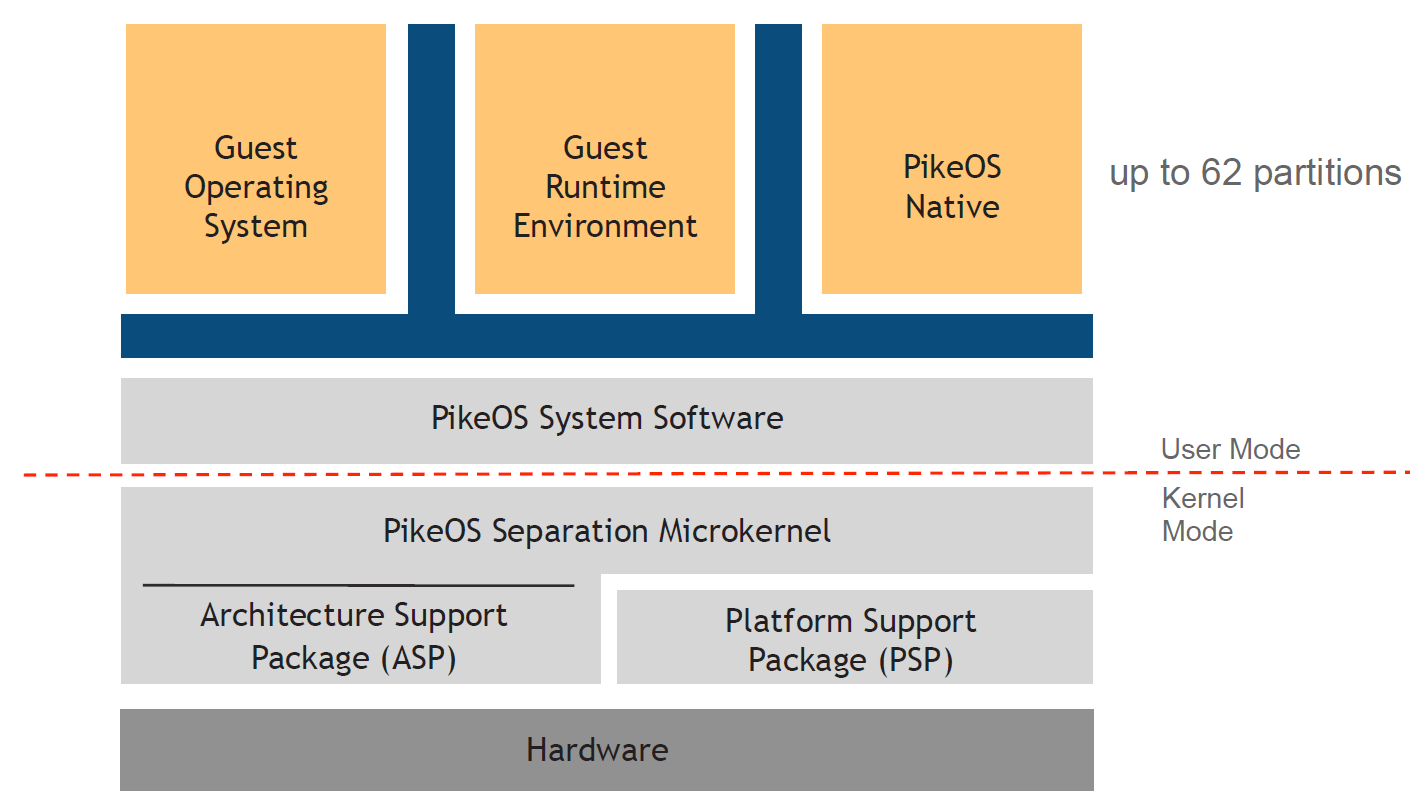
\includegraphics[width=1.0\textwidth]{PikeosArchitecture2}
\caption{PikeOS System Architecture}
\label{fig:pikeosarch}
\end{figure}

%\paragraph{} As an example of the use of guest personalities can be the use of Android, it is is being adopted for infotainment functions because they are a perfect fit for this Operating system. However, its openness and lack of security make it highly hackable, giving a \emph{'way in'} to the critical functions. Utilizing secure separation a designer may choose to host Android in open partition and separate it from the critical functions which are running in another partition. This also provides an evolutionary path whereby partitions can be added while leaving legacy software unchanged. 

\subsection{Resource Partitions}
Resource partitions are one of the basic security mechanisms to support multiple virtual machines on top of PikeOS. They can be thought of as containers within which applications execute. Partitions define the system resources that their applications can use and provide protection domains between different applications. For this reason, PikeOS partitions are also referred to as \emph{resource partitions} (fig.\ref{fig:pikeosExecEntities}). An application running in one partition is completely unaware of applications in other partitions, and cannot access resources to which it does not have explicit access permission. A partition can be stopped, restarted or reloaded with different applications without affecting other partitions. PikeOS supports up to 63 resource partitions. All resource partitions are created by the kernel at boot time.

\begin{figure}[htbp] 
\centering    
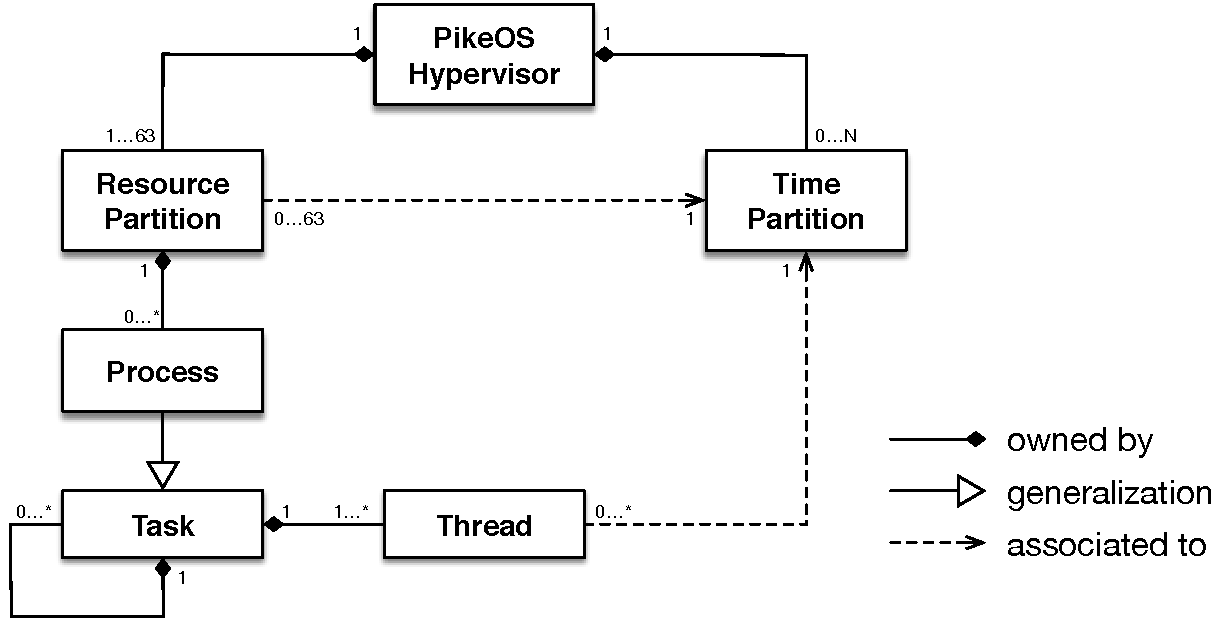
\includegraphics[width=1.0\textwidth]{PikeosExecEntities}
\caption{PikeOS Execution Entities}
\label{fig:pikeosExecEntities}
\end{figure}

\paragraph{} Resource partitioning is enforced by using the MMU to control access to the available resources. To access a resource, each hardware device is somehow represented by a physical address. Thanks to this, resource partitioning can be realized by forcing the MMU to map a certain memory area into a partitions virtual memory space and allow or deny read/write access to this memory space. The configuration of the MMU is done statically at system startup in the PikeOS microkernel and is not modifiable at run-time, also ensuring security. In summary, the separation makes sure that errors occurring in one partition cannot propagate to another partition.

\subsection{Processes and Tasks}
Inside a resource partition we can find different \emph{processes} that, from the kernel point of view, are PikeOS \emph{tasks} (see fig.\ref{fig:pikeosExecEntities}). Each process has its access rights to resources, including CPUs. The set of processors on which task threads can be scheduled, can be specified in the CPU mask attribute. 

\paragraph{} Moreover, each PikeOS task has a set of abilities associated with it, which the kernel uses to verify that the task’s threads have sufficient permissions to use certain kernel services. An ability is said to be enabled if the task is allowed to use the corresponding kernel service, and it is said to be disabled if the task is denied use of that service. Abilities are a task property, so all threads within a task share the same set of abilities.

\subsection{Threads}
Threads are the schedulable entities of a task. Each thread has it execution priority and, again, the affinity mask that express on which processors the thread can be scheduled. A thread may assume one of the following states (fig. \ref{fig:ThreadStates}):
\begin{itemize}
\item \emph{Inactive}. Threads in the INACTIVE state are never scheduled and are not valid targets for communications. When a task is activated, all threads are in the INACTIVE state. Also, a thread delete can put the target thread in this state.
\item \emph{Current}. A thread which owns the CPU is in the state. This thread (the current thread) can either execute user-level code or execute code inside the PikeOS kernel.
\item \emph{Waiting}. A thread is in this state if is waiting for a communication, an event, a resource.
\item \emph{Ready}. A is tread in this state if it is ready to continue its execution. Therefore is eligible to become the current thread.
\item \emph{Stopped}. A thread in this state is never eligible to become the current thread.
\end{itemize}

\begin{figure}[htbp] 
\centering    
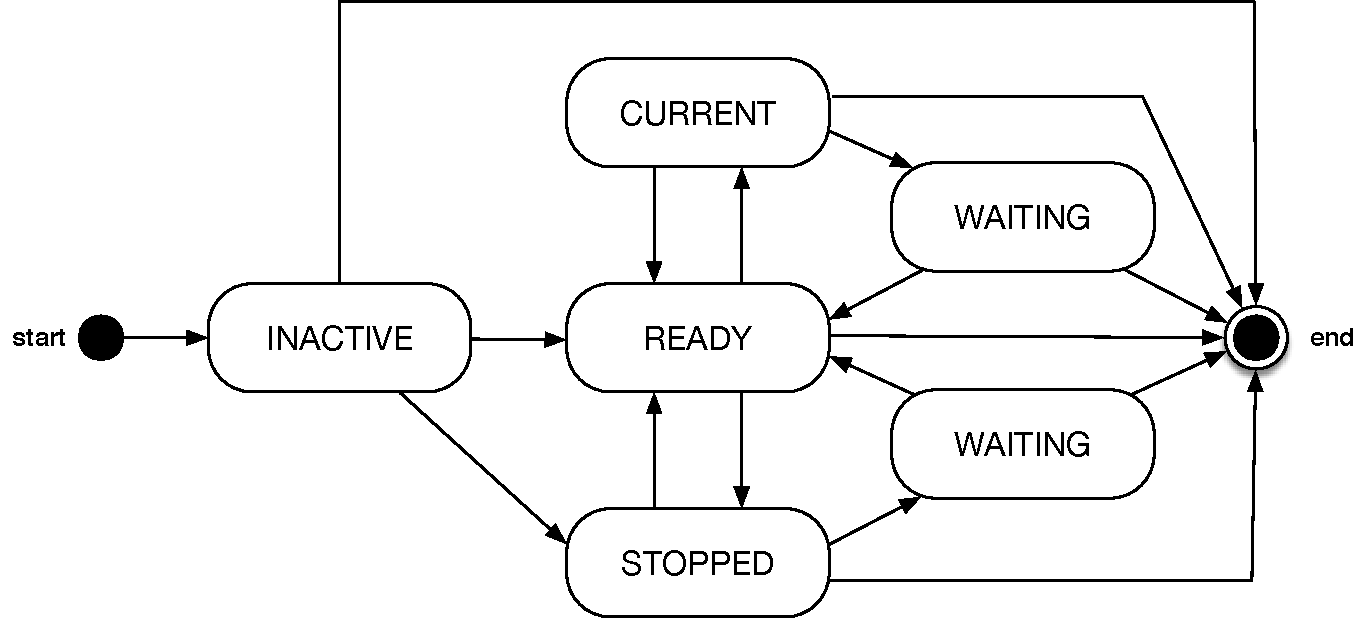
\includegraphics[width=1.0\textwidth]{ThreadStates}
\caption{PikeOS Thread States}
\label{fig:ThreadStates}
\end{figure}

A thread is put into the STOPPED state using p4\_thread\_stop().

\subsection{Time Partitions}
The PikeOS partition scheduler uses a combination of priority-based and time-driven scheduling. 
\par In contrast to the ARINC 653 standard, PikeOS scheduling uses a one-to-n assignment of resource partitions to time-partitions. This means that one or more resource partitions can be assigned to one time-partition. In this work, we use time partitioning to allocate a certain amount of CPU time to each resource partition (even though PikeOS capabilities go beyond this, this approach is fully ARINC 653 compliant). In this case, there is a \emph{one-to-one relationship between time and resource partition}s. This type of configuration is illustrated in figure \ref{fig:TimePartitioning}. Moreover, a PikeOS partition may host more than one task (Process), but in this work, we assign one task to one resource partition.
\paragraph{} Each Time Partition is made by one or more \emph{Time Windows} representing a time slice allocated to that Time Partition. Each Time Windows can be marked as the start of a new period, allowing a static definition of preemption between partitions.

\begin{figure}[htbp] 
\centering    
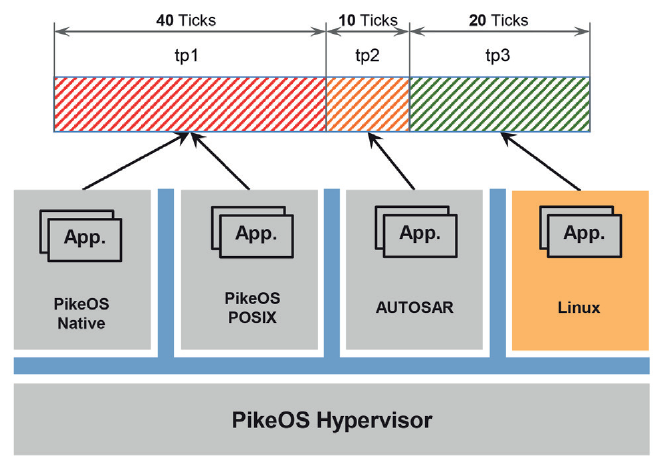
\includegraphics[width=0.8\textwidth]{TimePartitioning}
\caption{PikeOS Time Partitioning}
\label{fig:TimePartitioning}
\end{figure}

\paragraph{}It is worth mentioning that, in contrast to the ARINC 653 standard, one special partition, that is active at all times, exists. This time partition is referred as the \emph{background partition}\footnote{Background time-partition in parallel to the active
time-partitions is an invention by SYSGO and under active patents.}, \TP{0}, whereas the currently active one of the time-switched partitions is called the \emph{foreground partition}, \TP{i} with $i={1,...,N}$.

\subsection{PikeOS Scheduler}\label{sec:P4Scheduler}
Each time partition has its own priority, in addition to that, threads do also have a priority attribute. Whenever both the foreground and background partitions have active threads, the thread to be executed is selected according to its priority. Figure \ref{fig:PikeosScheduler} shows the principle of operation: each time partition is represented as a priority-sorted list of FIFO ready queues. Each of them delivers its highest priority ready thread and of these, the highest priority one from either \TP{0} or the currently selected \TP{i} gets chosen for dispatch.

\begin{figure}[htbp] 
\centering    
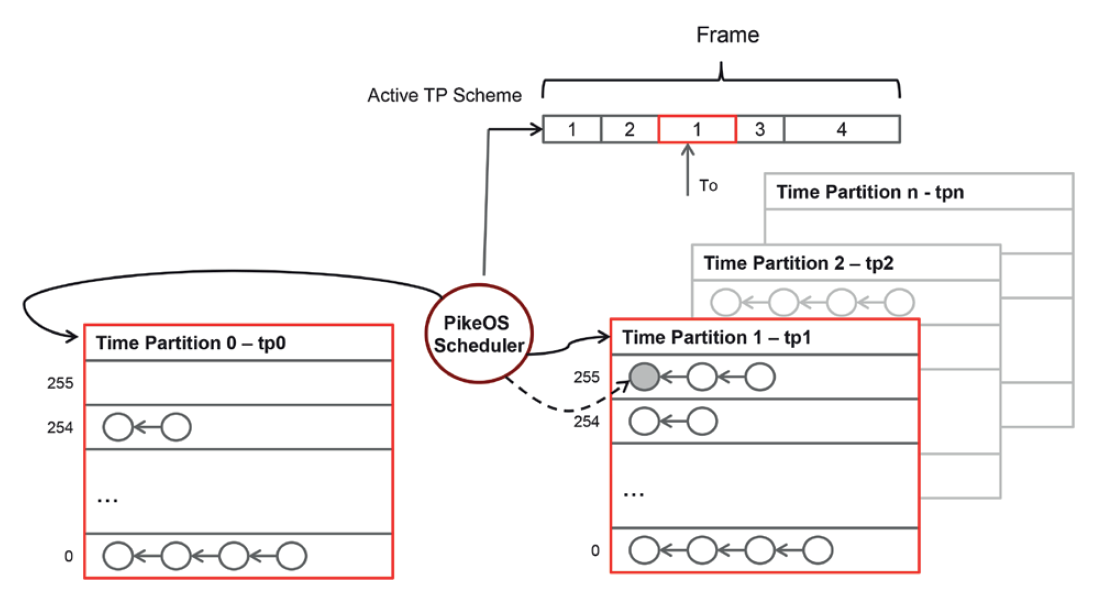
\includegraphics[width=1.0\textwidth]{PikeosScheduler}
\caption{PikeOS Time Partition Scheduler}
\label{fig:PikeosScheduler}
\end{figure}

\paragraph{} Partitions periodically receive guaranteed time slices. But, whenever one of these partitions completes its job prior to having consumed its entire time slice, the unused time automatically falls back to the next lower priority thread in the background time partition. Thus, by running explicitly non-real-time applications with lower priority threads in the background time partition (\TP{i}), these non- real-time applications receive all the computational resources that were assigned to, but not consumed by real-time application in the foreground partition (\TP{i}). This is a powerful approach to enforce the throughput of the safety-critical system. Figure \ref{fig:PikeosLowTP0}).

\begin{figure}[htbp] 
\centering    
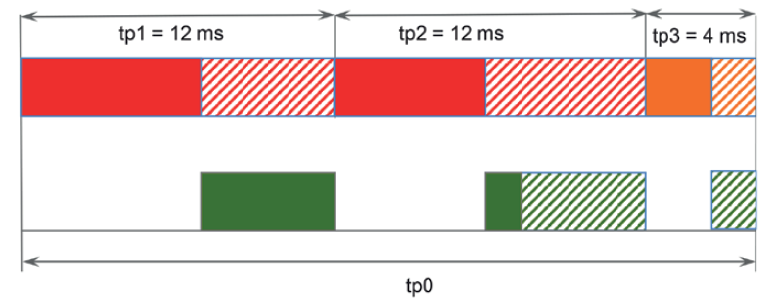
\includegraphics[width=0.7\textwidth]{PikeosLowTP0}
\caption{PikeOS Scheduling with low priority background application}
\label{fig:PikeosLowTP0}
\end{figure}

In the opposite scenario, it is possible to define threads in the background domain, which can override time partitioning by assigning them a priority above those of the foreground domain threads (fig. \ref{fig:PikeosHighTP0}). 

\begin{figure}[htbp] 
\centering    
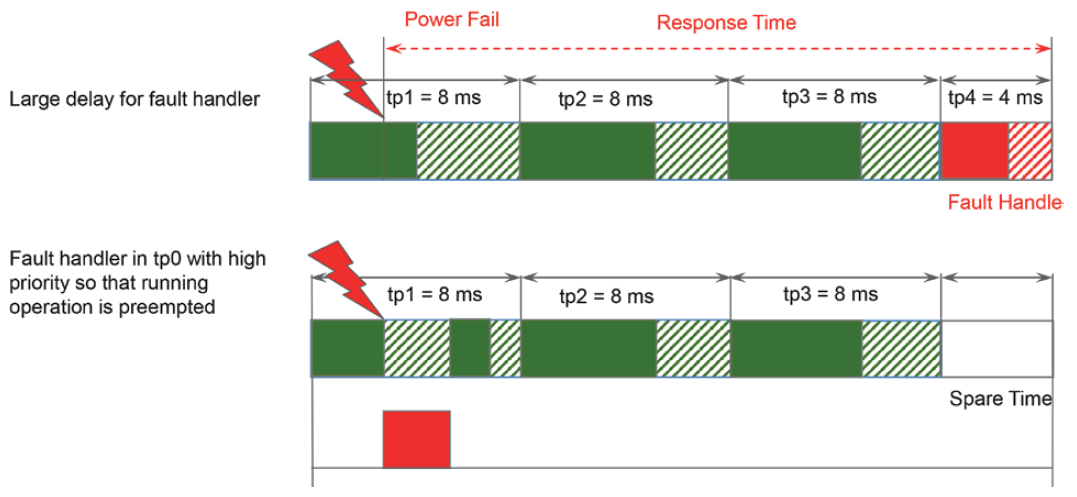
\includegraphics[width=1.0\textwidth]{PikeosHighTP0}
\caption{PikeOS Scheduling with with high priority background application}
\label{fig:PikeosHighTP0}
\end{figure}

\paragraph{}The upper time-diagram in Figure \ref{fig:PikeosHighTP0} has a fault handler, which is called in a dedicated time-partition \TP{4}. In case of a failure the response-time of the fault-handler can be quite high if the error happens right after the fault handler time-partition has ended. By assigning the fault handler to \TP{0}, the handler is starter immediately, as it has the highest priority among all active threads (lower time-diagram of Figure \ref{fig:PikeosHighTP0}). Clearly, such high priority threads must be considered as trusted code from the point of view of the threads that they can preempt.

\paragraph{} PikeOS support the possibility to change, at runtime, the Time Partition schedule. Each schedule is expressed (statically) inside the configuration file, and it is called \emph{scheme}. Schemes allow the system designer to adjust the time partitioning to handle exceptional situations rather than having to design a single time partitioning scheme which will suit all possible scenarios. The following XML code fragment shows a configuration with two schemes named "SCHED\_BOOT" (which is the one loaded at startup) and "SCHED\_POWERFAIL".
% CODE FRAGMENT
\lstinputlisting{Chapters/SrcCode/ScheduleScheme.xml}

\par Where the duration is expressed in \emph{Ticks}. Each Time Windows can be marked as a new period starting point just adding \emph{VM\_SCF\_PERIOD} its flags field.

\paragraph{} The PikeOS hypervisor provides means to invalidate instruction caches and TBLs and to flush the data cache between time partition switches (fig. \ref{fig:PikeosCacheFlush}). This ensures that caches and TLBs are in a defined state when a partition starts its execution. The cache/TLB flush and invalidate operation takes place during the time partition switch, so it will introduce a delay for the partition activation and thus cause a jitter. A possible approach to know the duration \cite{PikeosScheduling} of this delay is to define a small (but big enough) time partition window, which is allocated to an unused time partition ID and to insert this before the time critical application. This eliminates the jitter of the time critical application.

\begin{figure}[htbp] 
\centering    
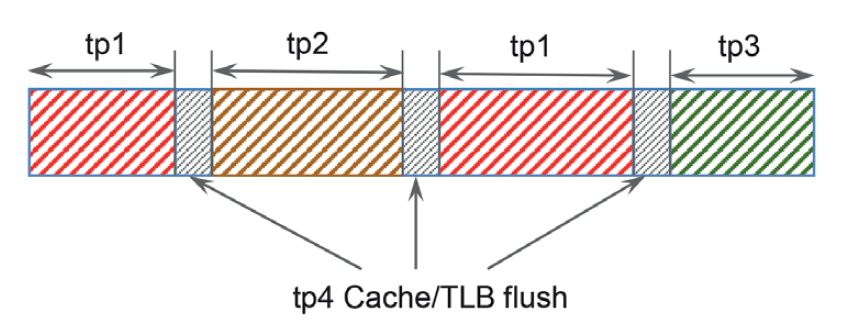
\includegraphics[width=0.8\textwidth]{PikeosCacheFlush}
\caption{PikeOS Cache and TLB Flushing}
\label{fig:PikeosCacheFlush}
\end{figure}

\subsection{Timeouts}
The PikeOS kernel provides a logical timebase for system time and timeouts. The system time value represents the elapsed time since startup. The resolution of the system time is platform and configuration dependent.

\par The PikeOS kernel provides different types of timeouts, in this work only \emph{Normal Timeouts} are used. They are timeouts that specifies a point in time with respect to the system time. Each timeout can be absolute or relative: an absolute timeout specifies the timeout as a system time value, while a relative timeout specifies the timeout as a difference relative to the current system time. Valid values are:
\begin{itemize}
\item \verb|P4_TIMEOUT_NULL|
\item \verb|P4_TIMEOUT_INFINITE|
\item numeric values
\end{itemize}

Expired timeouts are evaluated with a minimum frequency corresponding to the period of the system tick. Timeout expiration is checked before every rescheduling decision. A rescheduling is always evaluated when a system tick is processed by the kernel. However, the effective expiration depends on whether a time window of the caller's time partition is active or not. If the caller’s time partition is active, the timeout expires immediately. If no window of the caller’s time partition is active, the timeout does not expire when this time point is reached. The caller remains blocked, and the effective timeout expiration occurs when the caller’s time partition is next activated. In the first case, the thread may be scheduled immediately if it has the highest priority in the system. In the second case, the service call behaves as if the timeout did not expire.

\subsection{Communication primitives}\label{sec:CommPorts}
PikeOS provides message based communication through statically configured communication channels. A communication channel is a link between two ports, a \emph{source port} and a \emph{destination port}. The data flow is from the source port to the destination port – the view point is thus from the channel between the ports. The source and destination ports may be located within the same partition, within two different partitions, or within one partition and a port provider. In this work, we use communication ports mainly as an inter-partition communication mechanism. 

\paragraph{} The PikeOS  kernel provides two different types of port that allows different partitions to communicate, these are:
\begin{itemize}
\item \emph{Sampling Ports}. It uses a single message buffer that is atomically updated by a write operation; it also maintains the age of a message measured from the time of reception, which can be compared to the port’s refresh rate (this is used to derive a message validity);
\item \emph{Queuing Ports}. It operates as a FIFO buffer with a maximum message size.
\end{itemize}

\paragraph{}Communication via ports guarantees that either an entire message is written to or read from a port or no data is transferred at all. Queuing ports provide a blocking API with a message queue and with an optional timeout. Messages written to a queuing port are buffered within the PikeOS framework, i.e., they are copied twice: once on the write and once on the read. This ensures that a message that has been successfully written to a queuing port and cannot be corrupted by any user application, particularly not the sending one when it changes the send buffer. It is not an error for a port to be unconnected to another port. Instead, the port will behave as if the other side is completely unresponsive.

\paragraph{} Every channel must have exactly two endpoints: one source and one destination port. A queuing port can only belong to one channel. A destination sampling port can only belong to one channel, while a source sampling port can be referenced in an arbitrary number of channels. This allows a configuration where one source sampling port is connected to many sampling destination ports (1-to-n multicast). Summarizing, the main characteristics of a communication port (either Sampling or Queuing Port) are the following:
\begin{itemize}
\item Message Oriented (one message per transaction).
\item Channel establish port-to-port communication.
\item Queuing ports support blocking with timeouts, sampling ports provide the last valid data with validity (freshness) check.
\item Suitable for medium size data (data are copied twice).
\end{itemize}

\subsection{User Space Synchronization}\label{sec:spinlocks}
For synchronization between threads, PikeOS supports all the most common mechanisms including: \emph{Mutexes}, \emph{Condition Variables}, \emph{Barriers}, \emph{Semaphores} and \emph{Spinlocks}. All of these synchronization objects allow the calling thread to acquire and release objects and do not consume any kernel memory resources. Because we are focused on non-preemptive and highly deterministic behavior, the spinlock mechanism is the one that fits better.  
\par A spinlock causes the calling thread trying to acquire it to simply wait in a loop (\emph{spin}) while repeatedly checking if the lock is available. Since the thread remains active but is not performing a useful task, the use of this mechanism leads to a busy wait. Because they avoid overhead from operating system process rescheduling or context switching, spinlocks are very efficient if threads are likely to be blocked for only short periods and nonpreemptive behavior is accepted. In PikeOS, three API call are available for spinlocks handling:
\begin{itemize}
\item \verb|void p4_spin_init(P4_spin_t *lock)|: Initialize a spinlock to unlocked state.
\item \verb|void p4_spin_lock(P4_spin_t *lock)|: Acquire spin lock, spin in the contended case.
\item \verb|void p4_spin_unlock(P4_spin_t *lock)|: Release spin lock.
\end{itemize}

\subsection{Integration project}
\label{sec:IntegrationProject}
The configuration of a PikeOS system is mainly done in the integration project, i.e., configuration of all partitions, communication, permissions, etc., is done by the system integrator. The top-level tool for configuration is the Project Configurator. This tool is available as a command like tool as \verb|pikeos-projectconfigurator|, and as an Eclipse plugin as part of the graphical CODEO tool.

\begin{figure}[htbp] 
\centering    
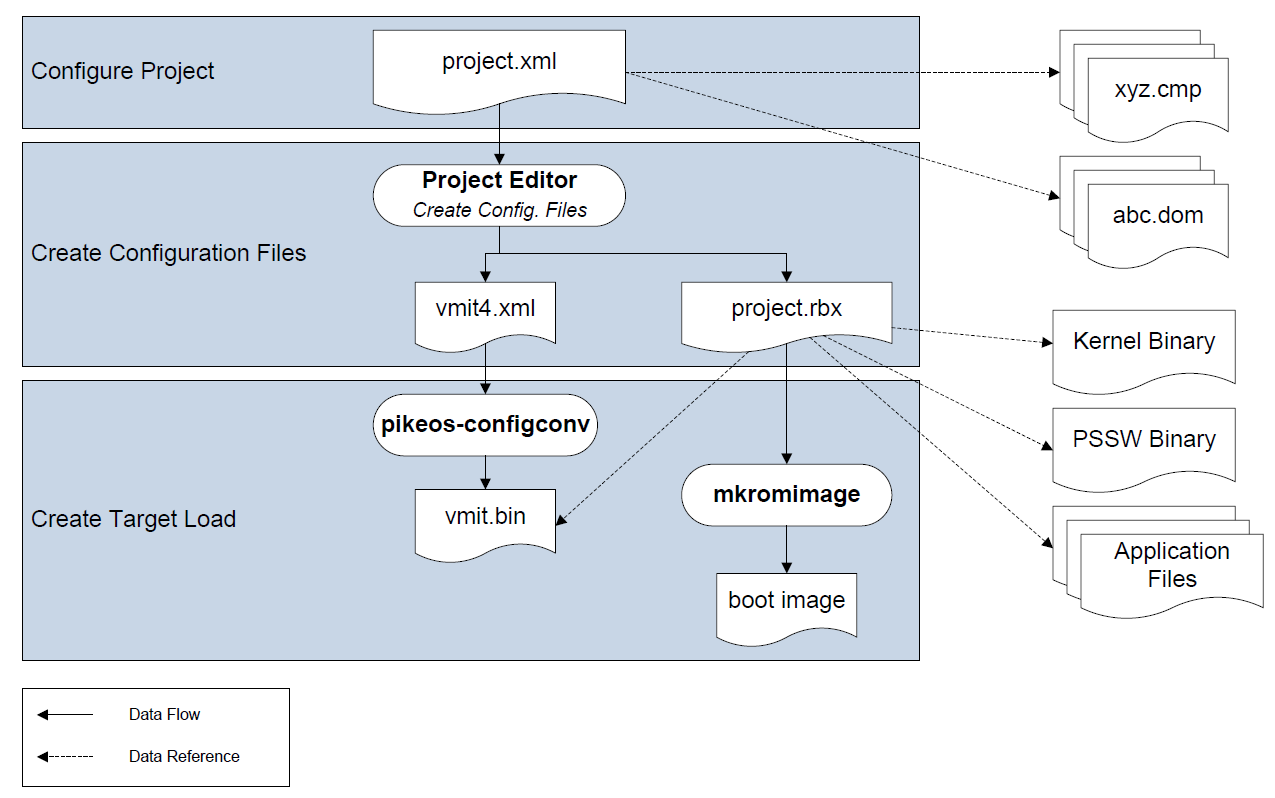
\includegraphics[width=1.0\textwidth]{PikeosProjectConfiguration}
\caption{PikeOS Project Configuration Overview}
\label{fig:PikeosProjectConfiguration}
\end{figure}

All the PikeOS relevant information are stored inside the \verb|project.xml| file. However, for lower level tools, the meta information inside this if file are not fully required; for that reason, the PikeOS Project Configurator converts the \verb|project.xml| file into the lower level configuration files used by the PikeOS system:
\begin{itemize}
\item \emph{ROM Boot Extended Configuration (RBX)} contains a description of the kernel, the memory region setup, the ROM file system and the file system;
\item \emph{Virtual Machine Initialization Table (VMIT)} contains all of the configuration settings of the PikeOS system and is used by the kernel to set up time and resource partitions as well as communication channels.
\end{itemize}
Both RBX and VMIT files are stored in XML format, but are converted to binary format before being loaded into the system.


%********************************** % Section  **************************************
\section{Simulink and Embedded Coder}
Simulink\textregistered \cite{Simulink}, developed by \emph{The MathWorks Inc.}, is a graphical programming environment for modeling, simulating and analyzing multidomain dynamic systems such as signal processing, control and communication applications. It supports system-level design, simulation, automatic code generation, and continuous test and verification of embedded systems. Thanks to its features, it is the \emph{de-facto} standard in model-based design.

\paragraph{} In order to generate C/C++ code from Simulink models, we can use \emph{Simulink Coder}\textregistered, formerly \emph{Real-Time Workshop}\textregistered. It supports code generation from both Simulink diagrams and Stateflow charts. Moreover; with Embedded Coder\textregistered, we can generate C/C++ code optimized to be used on embedded processors, on-target rapid prototyping boards, and microprocessors. It also provides traceability reports, code interface documentation, and automated software verification to assistance support standards such as DO-178 and ISO 26262 during development. It also supports external mode to connect the Simulink block diagram to the relative application that runs the model on the target hardware. The block diagram becomes a user interface to the real-time application, and by changing parameters in the Simulink blocks, the parameters in the real-time application also changes.

\subsection{Synchronous-Reactive Model of Computation}
Simulink implements a Synchronous-Reactive (SR) model of computation (MoC), it is designed for modeling systems that involve synchrony, a fundamental concept in concurrent systems \cite{Ptolemy2}. 
\par Synchronous-Reactive models are networks of Mealy-type blocks, eventually clustered into subsystems and can be continuous, discrete or triggered \cite{tres}. Continuous blocks process continuous-time signals and produce as output other continuous-signal functions according to the block description, typically a set of differential equations. Discrete-time blocks are activated at periodic-time instants and process input signals producing outputs signals and state updates. Finally, triggered blocks are only executed on the occurrence of a given event (a signal transition or a function call). 
\par Since we are interested in automatic code generation let us focus on discrete-time blocks which are (eventually) activated at each tick-time $t$. Let us denote a generic block $i$ as $B_i$, the input vector at tick-time $t$ as $\vec{u_i}(t)$ and similarly the output vector as $\vec{y_i}(t)$. Each block maintains a state vector $\vec{s_i}(t)$, then the behavior of $B_i$ can be modeled as an \emph{output update} function
\begin{equation}
\vec{y_i}(t)=f(\vec{u_i}(t),\vec{s_i}(t))
\end{equation}
and a \emph{state update} function
\begin{equation}
\vec{s_i}(t+1) = g(\vec{u_i}(t), \vec{s_i}(t))
\end{equation}
Often, the two update functions are considered as one:
\begin{equation}
(\vec{y_i}(t), \vec{s_i}(t+1)) = h(\vec{u_i}(t),\vec{s_i}(t))
\end{equation}

\paragraph{} A fundamental part of the model executable semantics are the rules dictating the evaluation order of the blocks. A block has a \emph{direct feedthrough} relationship between ports when the output port is controlled directly by the value of any input port signal. Any block with direct feedthrough relationship cannot execute until the block(s) driving its input has (have) executed. Therefore the set of topological dependencies implied by the direct feedthrough relationships defines a partial order of execution of the blocks. When the simulation starts, Simulink computes a total order of block execution compatible with the partial one.

\subsection{Real-Time Workshop Code Generation Process}
\label{sec:RTWGenerationProcess}
The Real-Time Workshop simplifies the process of building application programs. One of its features is automatic program building, which provides a standard means to create programs for real-time applications in a variety of host environments. It does this in a fully customizable way. The overall model build process is depicted in figure \ref{fig:RTWBuildProcess}.

\begin{figure}[htbp] 
\centering    
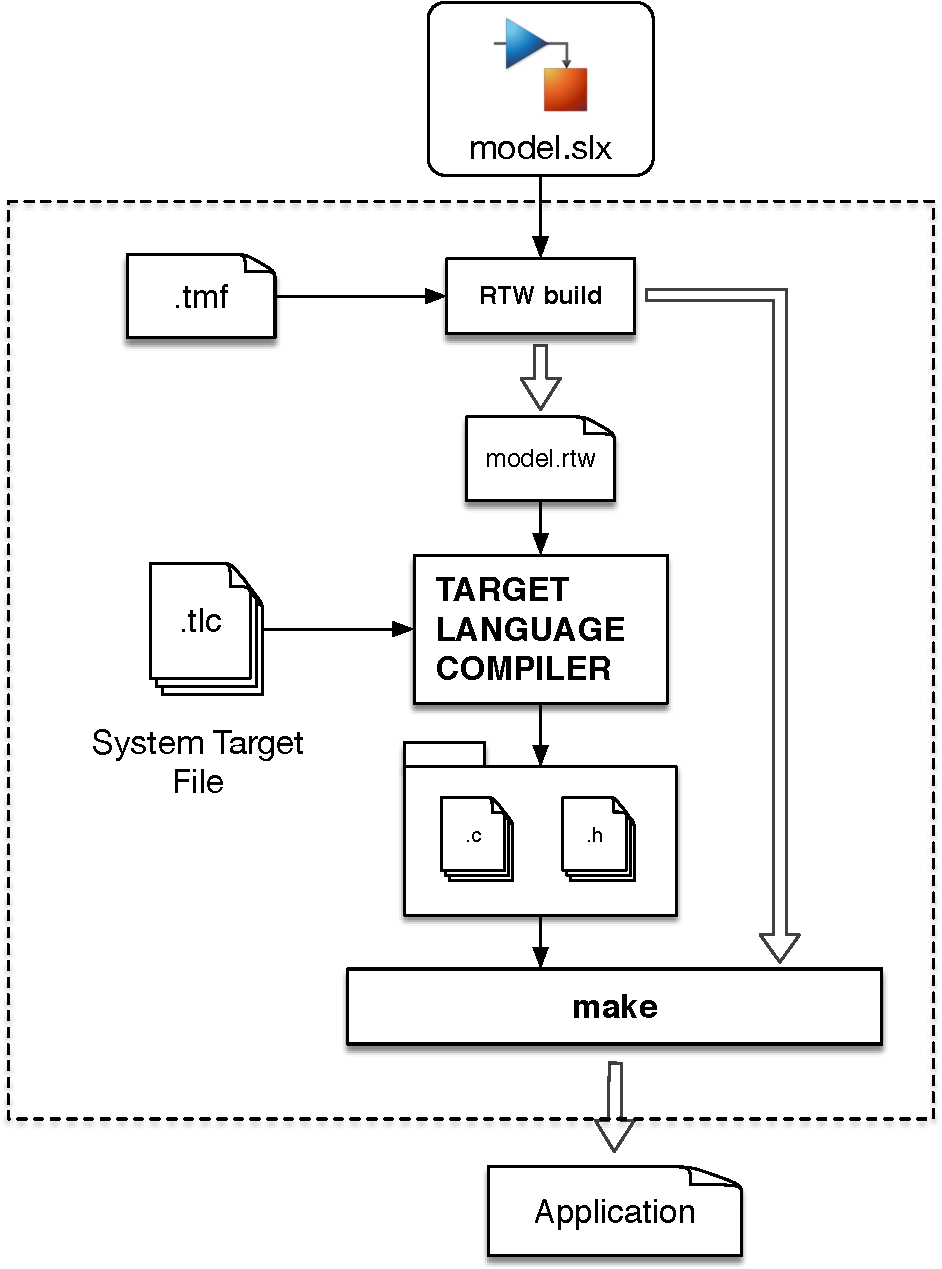
\includegraphics[width=0.45\textwidth]{RTWBuildProcess}
\caption{Real-Time Workshop Model Building Process}
\label{fig:RTWBuildProcess}
\end{figure}
The initial stage of the code generation process is to analyze the source model; the resultant description file, \verb|model.rtw|, it contains a \emph{compiled} representation of the model including a hierarchical structure of records describing systems, blocks, and their connections. This intermediate model description feeds the \emph{Target Language Compiler\textregistered} (TLC) that interprets it and guide the C/C++ code generation. It is also possible to write a \emph{Template Make File} (TMF) that define how to generate a Makefile for the actual compilation of the generated source files.

\paragraph{} The RTW file is a language-independent format, basically stored as an ASCII file. For example let us take a model like the one depicted in figure \ref{fig:RTWModelExample}. An excerpt of the generated \verb|model.rtw| is in figure \ref{fig:RTWFileExample}.

\begin{figure}[htbp] 
\centering    
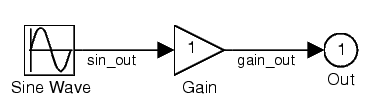
\includegraphics[width=0.4\textwidth]{RTWModelExample}
\caption{Model Example}
\label{fig:RTWModelExample}
\end{figure}

\begin{figure}[htbp] 
\centering    
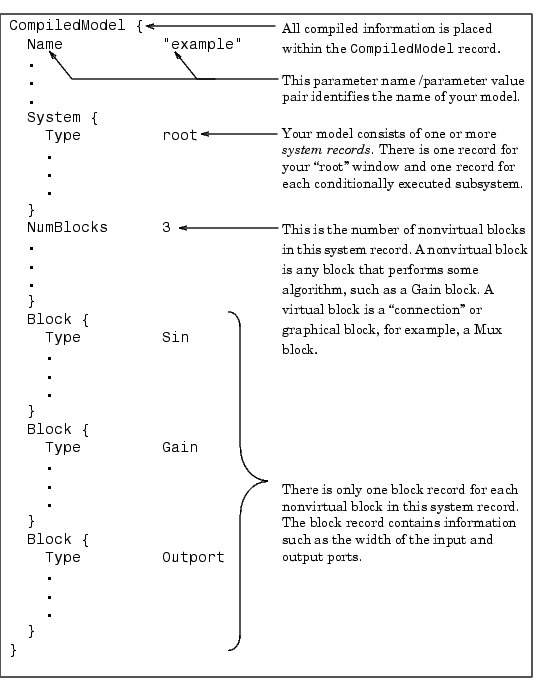
\includegraphics[width=1.0\textwidth]{RTWFileExample}
\caption{RTW File excerpt}
\label{fig:RTWFileExample}
\end{figure}

\subsubsection{Code Architecture}
\label{sec:CodeArchitecture}
When a model or a block is generated, RTW follows a general structure for the generated code. Blocks have inputs, outputs, parameters, states, and other general properties. All Block inputs and outputs are written into a block I/O structure (\verb|rtXX|) and instantiated as global variables. Figure \ref{fig:TLCCodeStructure} shows the general block data mappings.
\begin{figure}[htbp] 
\centering    
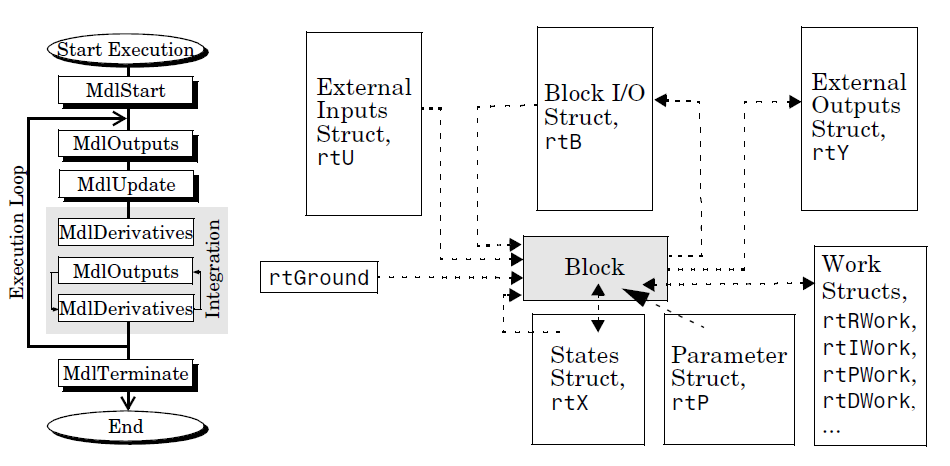
\includegraphics[width=1.0\textwidth]{TLCCodeStructure}
\caption{TLC Block code structure}
\label{fig:TLCCodeStructure}
\end{figure}
This structure apply also for the model when it is generated. Out of the generation process, three \emph{Entry Point Functions} are available:%Embedded Coder pag 702
\begin{itemize} 
\item \emph{model\_initialize}. Model initialization entry point.
\item \emph{model\_step}. Step routine entry point.
\item \emph{model\_terminate}. Termination entry point.
\end{itemize}
The structures and the function are stored in the source code. Embedded Coder creates a build folder in the working folder to store the following generated source code:
\begin{itemize} % pag 51 RTW UG OR pag 592 Embedded Coder UG
\item \emph{model.c}. Contains entry point functions implementing the model algorithm.
\item \emph{model\_private.h}. Contains local macros and local data that are required by the model and subsystems. This file is included in the model.c file as a \verb|#include| statement.
\item \emph{model.h}. Declares model data structures,a public interface to the model
entry points and data structures. This files is included in \verb|model.c| file.
\item \emph{model\_types.h}. Provides forward declarations for the data structure and the parameters data structure.
\item \emph{rtwtypes.h}. Defines data types, structures, and macros required by Embedded Coder generated code.
\item \emph{Optional files}. Sometimes also some source or header files are required by the generated code. These files are placed in the build folder.
\end{itemize}

\subsection{Concurrent Workflow}
Simulink provides a way to address the challenge of designing systems for concurrent execution through its \emph{Concurrent Workflow}. It uses the process of partitioning, mapping, and profiling to define the structure of the parallel application.
Partitioning enables to designate regions of the model as tasks. Mapping enables to assign partitions (tasks) to processing elements such as FPGAs or CPUs. Then Profiling simulates deployment of the application under typical computational loads.
\begin{figure}[htbp] 
\centering    
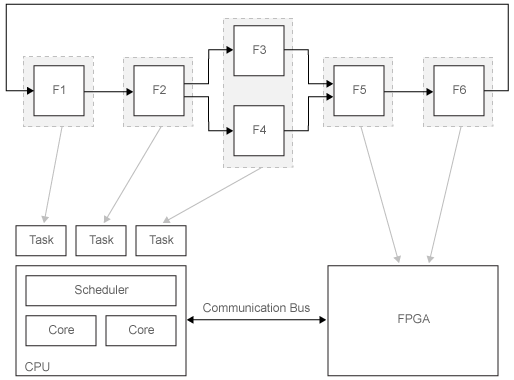
\includegraphics[width=0.8\textwidth]{SimulinkConcurrentWorkflow.png}
\caption{Simulink Multi-Core Partitioning}
\label{fig:SimulinkTaskPartitioning}
\end{figure}
%https://www.mathworks.com/help/simulink/ug/solving-embedded-performance-problems-using-multicore-processors-and-fpgas.html
%https://www.mathworks.com/help/simulink/ug/implicit-and-explicit-partitioning-of-models.html
\par Partitioning is the first step for defining the application's structure. There are two ways to partition the model for running on individual processing nodes.
The automated way of creating tasks and mapping them to processing nodes is called \emph{implicit partitioning}. Simulink partitions the model basing on the sample times of blocks at the root level. Each sample time in the model corresponds to a partition, and all blocks of a single rate or sample time belong to the same partition. Then these partitions are mapped to tasks and their priority assigned according to rates. Therefore, implicit partitioning assumes the hardware architecture consists of a single multi-core CPU and that the Operating System scheduler handles all the execution according to task priorities.
\par Another way to specify partitions is to use \emph{explicit partitioning}. In explicit partitioning, partitions are created in the root-level model by using \emph{referenced models} (fig. \ref{fig:SimulinkTaskProfiling}). For example, if the model is made by a data acquisition and a controller, a possible partitioned model puts these components in two difference referenced models at the model root-level. Each sample time in a referenced model or a system block is a partition. Then using the \emph{Model Configurator}, in the Concurrent Execution dialog box, each task can be mapped to one processing node (set the affinity mask).
%https://www.mathworks.com/help/simulink/ug/implement-task-parallelism-in-simulink.html
\begin{figure}
  \begin{subfigure}{0.65\textwidth}
    \centering
    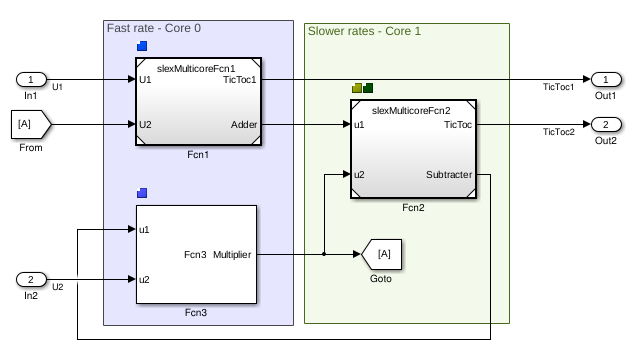
\includegraphics[width=1\textwidth]{slexMulticorePartitioning}
    \caption{Simulink Explicit Partitioning}
    \label{fig:slexPartitioning}
  \end{subfigure}%
  \begin{subfigure}{0.35\textwidth}
    \begin{subfigure}{\textwidth}
      \centering
      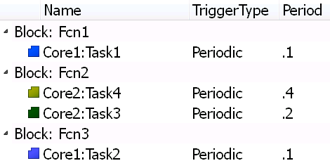
\includegraphics[width=1\textwidth]{slexMulticoreMapping}
      \caption{Simulink Mapping}
      \label{fig:slexMapping}
    \end{subfigure}
  \end{subfigure}
  \caption{Simulink Concurrent Workflow (by \emph{The Mathworks})}
  \label{fig:SimulinkTaskProfiling}
\end{figure}

\paragraph{} This tool is not yet mature, and complex to customize, for this reason, does not suit well for mixed-critical applications. The aim of both implicit and explicit partitioning is the extraction of tasks by grouping blocks instead of finding a way to isolate functionalities (robust partitioning). The automatic partitioning and mapping do not address the problem of safety and secure code execution. Instead, it focuses only on performance without any optimization. Even with explicit partitioning and mapping task priority assignment is rate-monotonic (tasks with shorter rate results in a lower priority) and does not take into account Worst-Case Execution Time of tasks and Resource usage. Both this two information are critical for schedule tasks minimizing interferences while exploiting as much as possible the task parallelism. Moreover, the whole process is strictly tied with Simulink environment making difficult to integrate pieces of software developed by hand or automatically generated by other software.

\paragraph{} For overcoming all these limitations, one possible approach is to customize the code generation process. Simulink provides a configuration tool for this: the \emph{Target Language Compiler}. The following section briefly introduces it.

\subsection{Target Language Compiler}
The Target Language Compiler tool is part of the Real-Time Workshop. It enables the customization of the C/C++ code generated from any Simulink model or custom defined blocks. It has been designed for the purpose of converting the model description file, \verb|model.rtw|, into target-specific code.

\paragraph{} After reading the rtw file, the Target Language Compiler generates its code based on \emph{target files}, which specify any particular code for each block and the overall code style. TLC works like a text processor, it has mark-up syntax similar to HTML, along with the power of scripting languages, plus the data handling power of MATLAB (TLC can invoke MATLAB functions). All Simulink blocks are automatically converted to code (except MATLAB function blocks and S-function blocks that invoke M-files). 
\par In order to create a target-specific application, Real-Time Workshop also requires a template makefile that specifies the appropriate C compiler and its options for the build process. The template makefile is then transformed into a makefile (\verb|model.mk|) by performing \emph{token expansion} specific to a given model.

\paragraph{} Any rtw file contain a series of (usually hierarchically nested) \emph{records} in the form:
\begin{verbatim}
recordName {itemName itemValue}
\end{verbatim}
Item names are alphabetic. Item values can be strings or numeric values ( including scalars, vectors, and matrices). Curly braces set off the contents of each record, which may contain one or more items, delimited by space, tab, and/or return characters.
\par In rtw file automatically generated from a Simulink model, the top-level (first) record’s name is \verb|CompiledModel|. Each block is represented by a subrecord within it, identified by the block’s name. The TLC, however, can parse any well-formed record file. For example, we can access:
\begin{lstlisting}
%% In tlc file you can:
/* Print a comment in the output file */
%assign genDate = CompiledModel.GeneratedOn
The Model Name is: <%CompiledModel.Name>
Generated on: %<genDate>
\end{lstlisting}
The first line is a comment; all text on a line following the characters \verb|%%| are treated as a comment (ignored, not interpreted or output). The text on the second line is printed out in the file as it is.
\par The third line execute a TLC directive (because it starts with \verb|%|), the directive \verb|assign| creates a variable named \verb|genDate| and assigns a string value to it. The \verb|%assign| directive creates new and modifies existing variables. Its general
syntax is:
\begin{verbatim}
%assign [::]variable = expression
\end{verbatim}
The optional double colon prefix specifies that the variable being assigned to is a global variable. In its absence, a local variable in the current scope is created or modified.
\par The last two line evaluates (expands) records. More precisely, in the first case, it evaluates the field called \verb|Name| existing in the scope called \verb|CompiledModel|. The syntax \verb|%<expr>| causes expression \verb|expr| (which can be a record, a variable, or a function) to be evaluated. This operation is sometimes referred to as an \emph{eval}.

\paragraph{} The previous does not print anything, because all outputs were directed to a null device (sometimes called the “bit bucket”). There is always one active output file, even if it is null. To specify, open, and close files:
\begin{verbatim}
%openfile streamid [="filename"] [, mode]
%closefile streamid
%% Output operations ...
%selectfile streamid
\end{verbatim}
The \verb|%openfile| directive creates a file/buffer (in “w” mode), or opens an existing one (in “a” or “r” mode). Note required equals sign for file specification. Any number of streams can be open for writing, but only one can be active at one time. The directive is useful to switch between open files; they do not need to be closed until output operations to them are actually ended. When activated, \verb|STDOUT| directs output to the MATLAB command window.

\paragraph{} The \verb|%with| and \verb|%endwith| directive eases the burden of correctly coding TLC scripts and to clarify their flow of control. Syntax is
\begin{verbatim}
%with RecordName
%% TLC stamements...
%endwith
\end{verbatim}
they can also be nested; for example it can be very useful while using \verb|foreach| loops
\begin{lstlisting}
%with CompiledModel
%with DataTypes
%foreach dt=NumDataTypes
Data Type Index = %<dt>
Data Type Name: %<DataType[dt].SLName>
%endforeach
%endwith
%endwith
\end{lstlisting}

\subsubsection{Counting Blocks and Subsystems}
As an example, the following TLC code count subsystems and blocks in the model.
\begin{lstlisting}
%% File: CountSubSysAndBlocks.tlc
%% Count blocks and subsystems of a model.rtw file
%%
%% NOTE: Change "<matlabroot>/" below to the
%% MATLAB main directory on your system
%addincludepath "<matlabroot>//rtw//c//tlc//lib" %%Enables TLC to find included files
%assign Accelerator = 0 %%Needed to avoid error in utillib
%include "utillib.tlc" %%Inserts one file in another, as in C (not used here)
%selectfile STDOUT
*** SYSTEMS AND BLOCKS IN RECORDFILE
%assign nbls = 0
%with CompiledModel
%foreach sysIdx = NumSystems
%with System[sysIdx]
%assign nbls = nbls + NumBlocks
*** %<NumBlocks> blocks in system %<sysIdx + 1>
%endwith
%endforeach
*** recordfile contains %<nbls> blocks in %<NumSystems> systems
%endwith
*** END LISTING
%% end CountSubSysAndBlocks.tlc
\end{lstlisting}
we can run this script writing in the command window
\begin{verbatim}
tlc -r model.rtw CountSubSysAndBlocks.tlc
\end{verbatim}
obtaining, for example
\begin{verbatim}
*** SYSTEMS AND BLOCKS IN RECORDFILE
*** 8 blocks in system 1
*** 10 blocks in system 2
*** 4 blocks in system 3
*** 7 blocks in system 4
*** 17 blocks in system 5
*** recordfile contains 46 blocks in 5 systems
*** END LISTING
\end{verbatim}


%********************************** % Section  **************************************
\section{Developed Framework}\label{sec:DevelopedFramework}
The aim of the thesis is to develop a framework to run different applications with different criticality levels in multi-core platforms ensuring adequate safety requirements. While a robust partitioning and scheduling algorithm are still open problems, we focused on developing a code generation framework to implement, on PikeOS, such scheme.
\par For this reason, we first developed a complete but trivial partitioning and a scheduling algorithm that extracts information from a Simulink model, let the designer configure and run the optimization engine for threads allocation. This generates a configuration useful for the automatic code generation process. Figure \ref{fig:FrameworkOverview} shows the simplified design flow.
\begin{figure}[htbp] 
\centering    
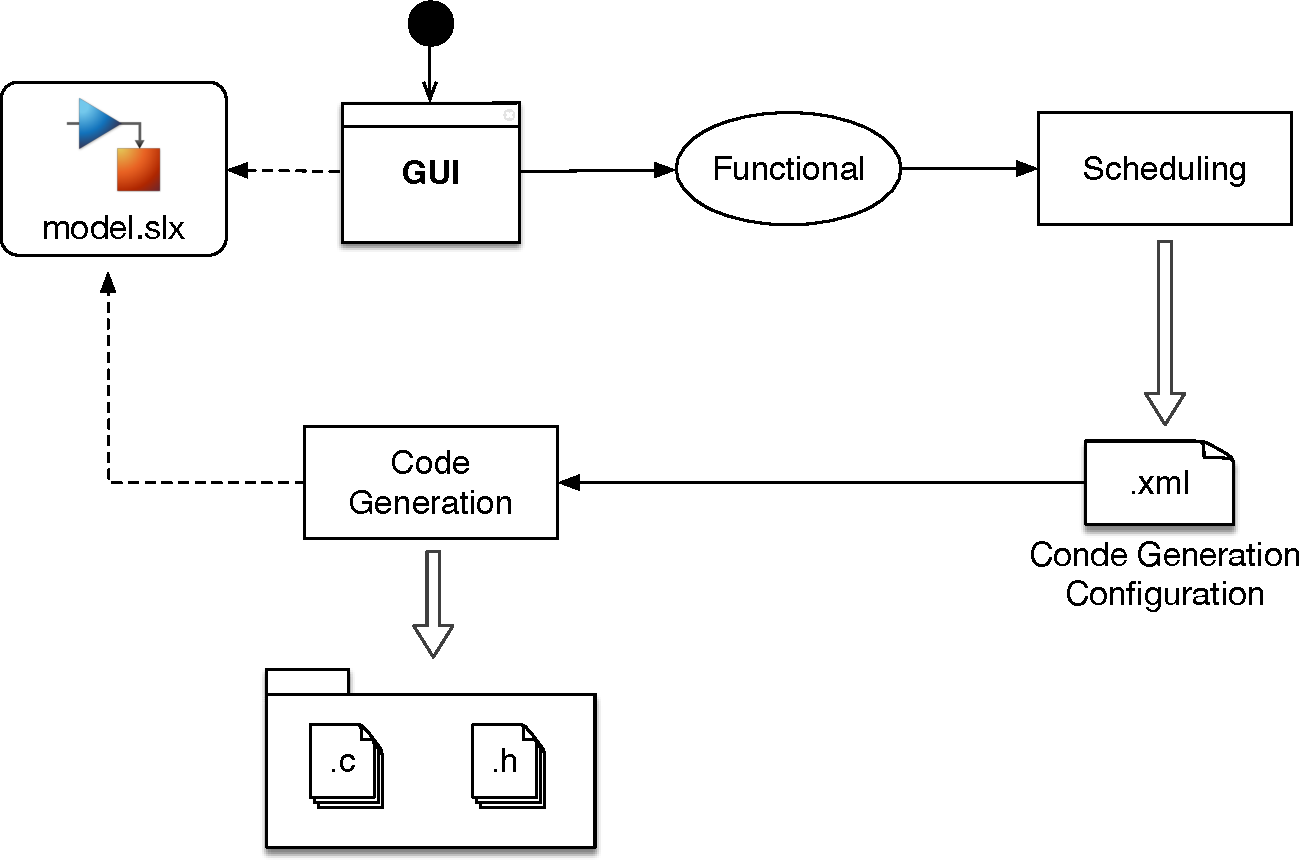
\includegraphics[width=0.7\textwidth]{FrameworkOverview}
\caption{Developed Framework overview}
\label{fig:FrameworkOverview}
\end{figure}
\par Once the models are developed and the simulation results are satisfactory, the system designer groups blocks in subsystems, which are considered as the unit of execution, such that there are no spare blocks among subsystems. Then a Matlab script uses the Simulink modeling API (programming interface) to parse the model structure and create a functional representation of the model to be utilized in the scheduling process (eventually exported an XML). Finally, if the scheduling gives good results, the code generation process can be started.

\subsection{Model Functional Representation}
A current challenge in the development of parallel applications is the achievement of a good scalability with the number of threads and processors. Often the scalability is heavily reduced by the precedence order of execution among threads (usually due to data dependencies). A possible approach to model the problem is through a \emph{Directed Acyclic Graph} (DAG). The DAG is a functional representation of the model, it consists of vertices (threads) and edges (communications/precedences) among nodes, with each edge directed from one vertex to another. The fact that it is an acyclic graph ensures that there is no \emph{algebraic loop} in the model. An algebraic loop occurs when a signal loop with only direct feedthrough blocks within it exist.
\par The designer can also add additional information to each node/thread such as
\begin{itemize}
\item Worst Case Execution Time (WCET) after performing some timing analysis on the subsystems\footnote{the subsystem will become a task, so this is the execution time related to a task.}. 
\item Criticality Level (A to E).
\item Resource Usage (a piece of resource like Shared Memory, UART, Ethernet, etc. can be defined and assigned to one or more threads).
\end{itemize}
This information is used by the engine to properly schedule threads on cores.
\par The functional model is created by a Matlab script that uses the Simulink modeling API (programming interface) to parse the model structure and create the DAG. It is based on the work of Matteo Morelli \cite{MorelliSee}. The Simulink model must comply with the restriction that:
\begin{enumerate}
\item The model consists of a collection of subsystems, with no spare blocks among them.
\item There are no continuous time blocks.
\item There are no multi-rate subsystems.
\end{enumerate}
These restrictions are a result of the fact that a C implementation should be generated from the model. 

\subsection{Partitioning and Scheduling Optimization}
The DAG represents a \emph{precedence graph} among threads, so it imposes a partial order of execution. To automatically generate an implementation (code generation) we must compute a total order among threads. This gap is an opportunity to improve safety and predictability (determinism) through partitioning and scheduling.

\paragraph{} In order to perform a real-time scheduling for the asks on multiprocessor platforms there exist two basic approaches: the \emph{partitioned approach}, in which each task is statically assigned to a single processor and migration is not allowed, and the \emph{global approach}, in which tasks can freely migrate and execute on any processor. Works from Gracioli\cite{Gracioli2013} and Melani\cite{Melani} shows a comparison of global scheduling and partitioned scheduling. Even though the global scheduling has several advantages, this thesis is focused on partitioned scheduling because the global scheduling would lead to preemptions and migrations, which produce more overheads and less determinism. In particular the latter might cause certification issues and this thesis wants reduce this possibility.

\par In this thesis we propose a general framework for a partitioned scheduling that can be mapped on PikeOS execution entities. For this purpose we identified several phases:
\begin{enumerate}
\item Mapping execution unit to tasks.
\item Task partitioning.
\item Task scheduling.
\item Priority assignment.
\item Partition scheduling.
\end{enumerate}
The scheduling process is implemented in Matlab as shown in figure \ref{fig:SchedulingProcess}.
\begin{figure}[htbp] 
\centering    
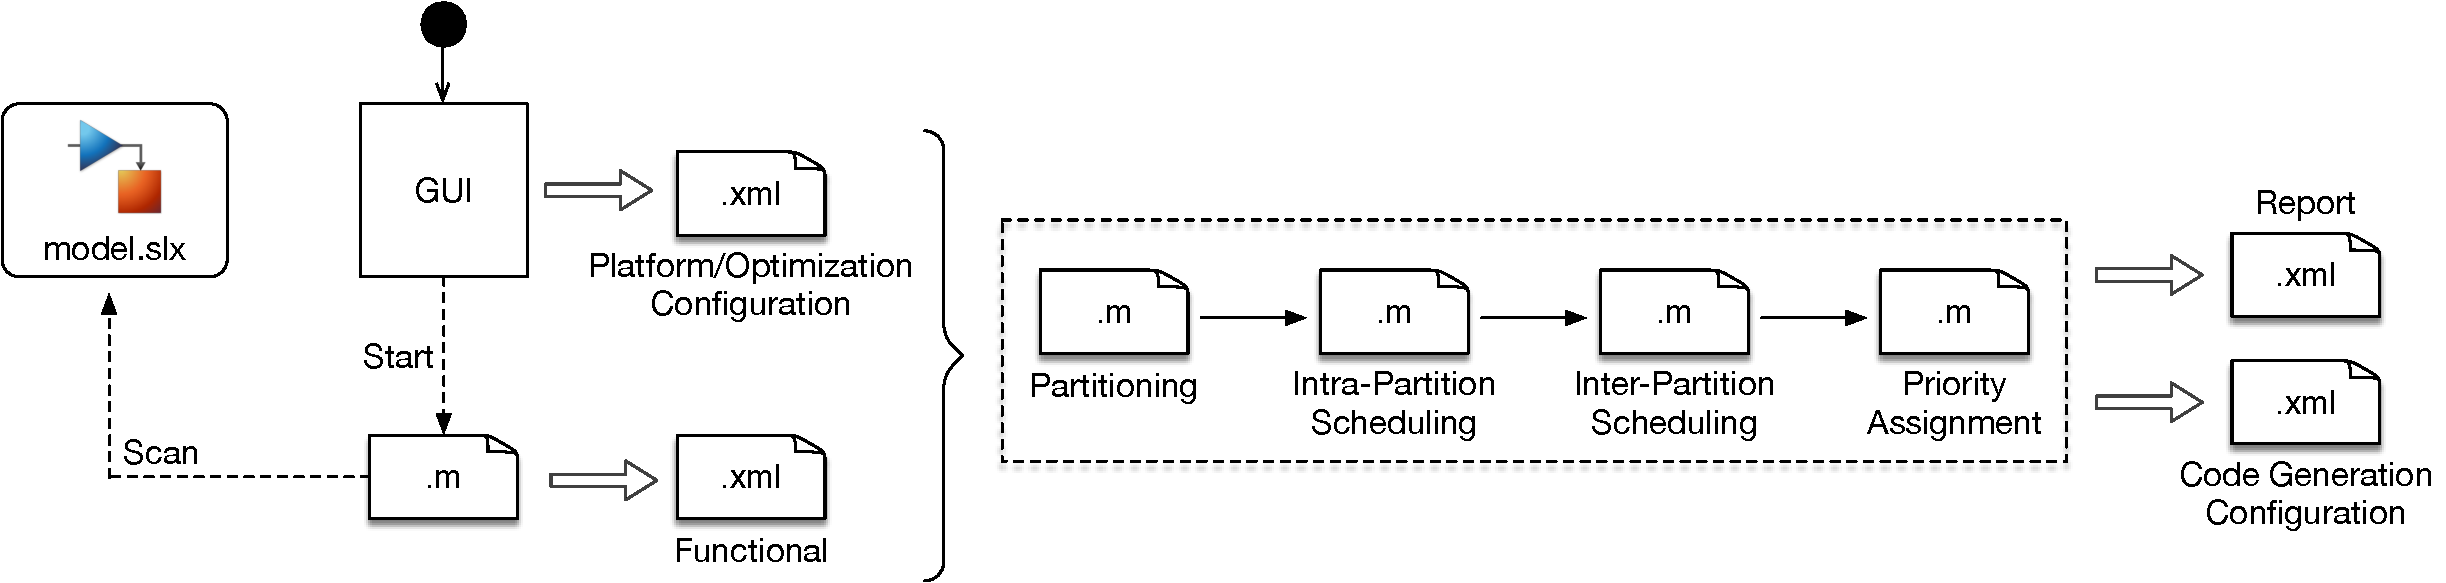
\includegraphics[width=1.0\textwidth]{SchedulingProcess}
\caption{Scheduling algorithm process}
\label{fig:SchedulingProcess}
\end{figure}

\subsection{Code Generation}
Code generation is a popular and mature technology. However, an optimal solution for code generation for mixed-criticality systems has not be found. Since robust partitioning is the common way to address mixed-criticality the code generation framework should take as input the description of such partitioned system. Recalling the fact that the code needs to be mapped into PikeOS execution entities, it is assumed that (with respect to PikeOS terminology) each Resource Partition is made by one Process with its threads and assigned to only one Time Partition. Obtaining the software architecture depicted in figure \ref{fig:SWArchitecture}.
\begin{figure}[htbp] 
\centering    
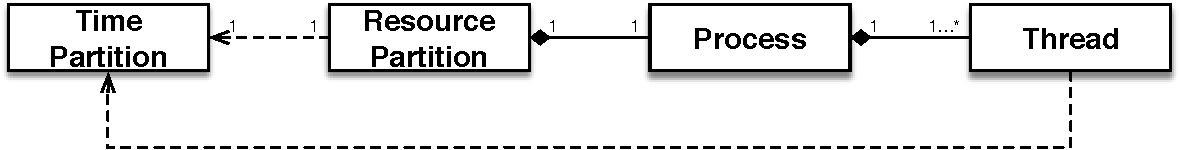
\includegraphics[width=0.9\textwidth]{SWArchitecture}
\caption{Software Architecture in the Developed Framework}
\label{fig:SWArchitecture}
\end{figure}
The reason why this architecture is proposed is that a different one would introduce further synchronization issues and less determinism. For example splitting a process in two separate processes, both assigned to the same resource partition would increase the possible interleaving among threads (basically all the possible states) and more synchronization calls for the communication. Moreover, since two processes (even if they are in the same Resource Partition) do not share the same virtual address space, more channels or additional shared memory regions must be defined. The same issues are caused if more than one Resource Partition is assigned to the same Time Partition.

\paragraph{} The underlying idea is to create a heterogeneous code generator partially independent from the platform. Since in this work the model representation is the Simulink Model, the code generation process is divided in two steps: \begin{enumerate}
\item Subsystems adaptation and generation: during this step Subsystem communications are eventually mapped to the right primitives (as defined in the code generation configuration file) and each Subsystem is generated with the Real Time Workshop/Embedded Coder as independent code.
\item System target code generation: here all the subsystems are glued together as threads, processes and partitions with target specific code.
\end{enumerate}
It can be noticed that the first step is OS agnostic if the communication primitives are an abstraction of the Operating System ones. The resulting code generation process is depicted in figure \ref{fig:CodeGenerationProcess}.
\begin{figure}[htbp] 
\centering    
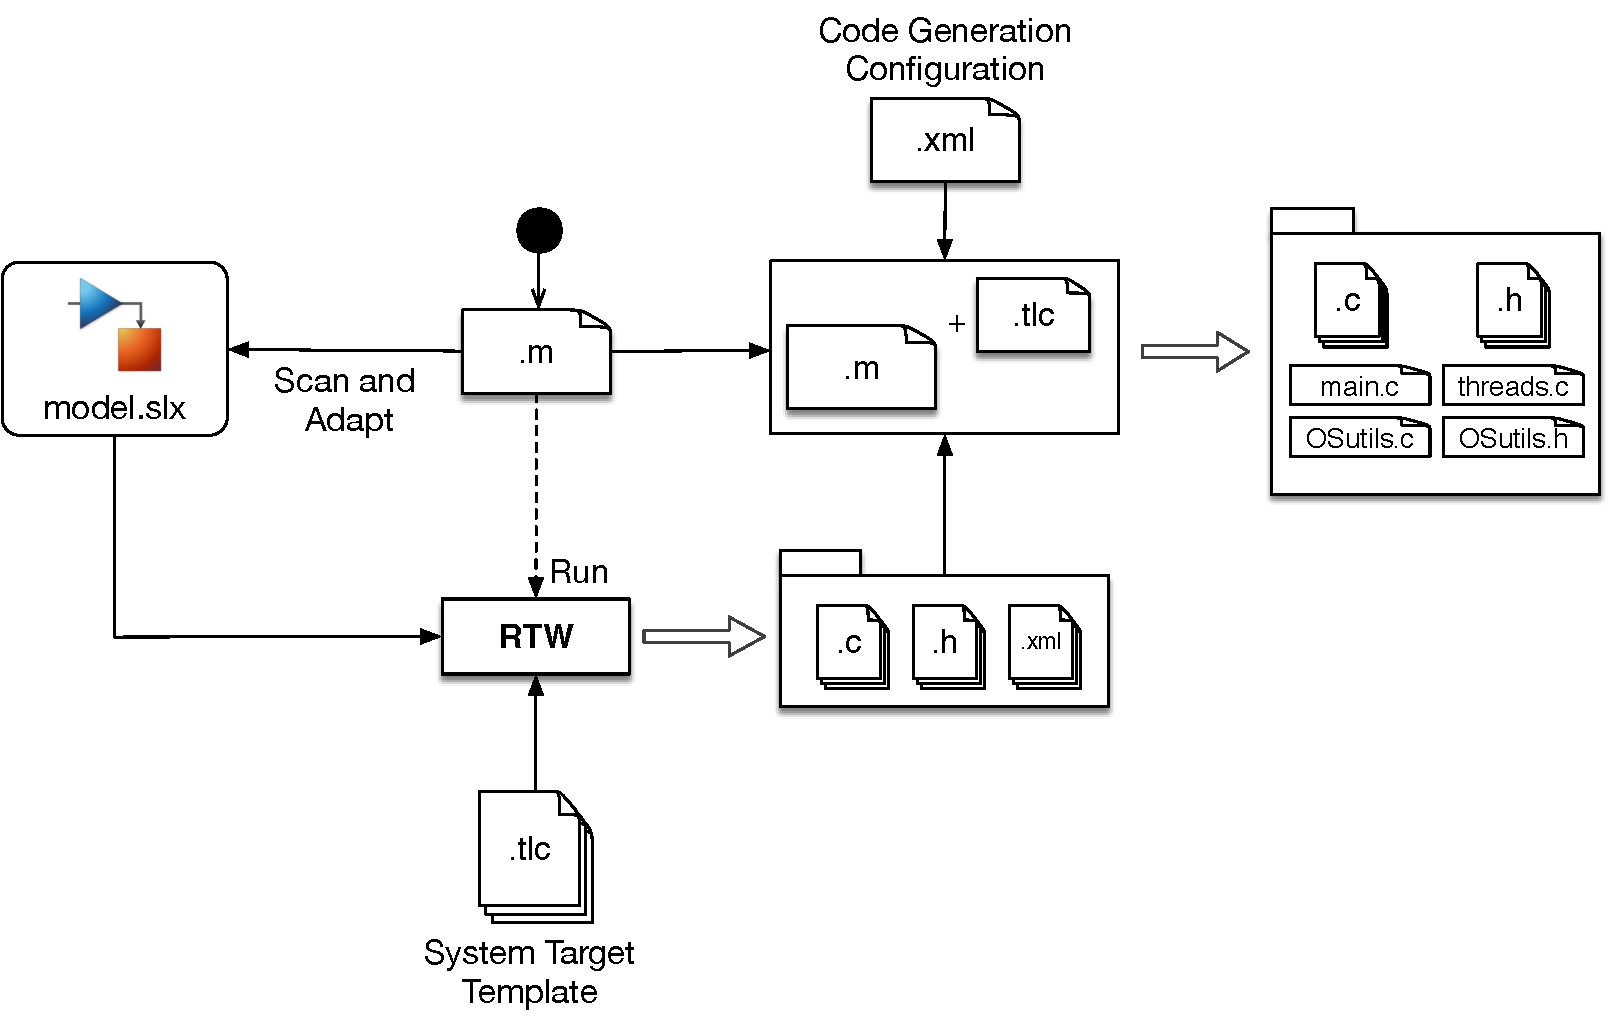
\includegraphics[width=0.8\textwidth]{CodeGenerationProcess}
\caption{Code generation process}
\label{fig:CodeGenerationProcess}
\end{figure}


% ~~~~~~~~~~~~~~~~~~~~~~~~~~~~~~~~~~~ % NTOES  ~~~~~~~~~~~~~~~~~~~~~~~~~~~~~~~~~~~
% The system runs different applications with different criticality levels, to reduce software complexity PikeOS is equipped with ARINC-653 compliant resource partitioning. The idea is to establish subsets of system resources, so-called “partitions”, serving as fault container: each program can only access its partition's own set of resources, so programs running in separate partitions cannot interfere with each other. Therefore, they do not need to trust each other and individual criticality levels can be assigned to each of them independently.
%PikeOS has been designed for use in safety-critical applications and has gone through a comprehensive validation according to safety standards like DO-178B, EN 50128, IEC 62304, IEC 61508,  ISO 26262, IEC 61513 for either the avionics, automotive, railway, medical, industrial automation or nuclear power plants. Since only the micro-kernel runs in privileged mode, all of its code contributes to the trusted code base of every application that might run on top of it. The effort of certifying a program is roughly proportional to the amount of code to be examined. This comprises the code of the program itself, but also that of the run-time environment (i.e. operating system, libraries etc.) which the program relies on. Therefore, the PikeOS micro-kernel consists of less than 10,000 lines of code making certification less expensive than that of conventional monolithic real-time operating systems. Even better: PikeOS allows the combination of applications of different levels of criticality where every application can be certified independently from others.

% https://www.sysgo.com/solutions/safety-security-certification/iso-26262/

%http://radio.feld.cvut.cz/matlab/toolbox/rtw/rtw_ug/tech_ov6.html